\documentclass[10pt, conference, letterpaper]{IEEEtran}

\usepackage{amsfonts}
\usepackage{amsmath}
\usepackage{amssymb}
\usepackage[utf8]{inputenc}
\usepackage[T1]{fontenc}
\usepackage{xcolor}
\usepackage{mathtools}
\usepackage{graphicx}
\usepackage{caption}
\usepackage{subcaption}
\usepackage{multirow}
\usepackage{booktabs}
\usepackage{cite}
\usepackage{bm}
\usepackage{tikz}
\usetikzlibrary{positioning, arrows.meta, shapes.geometric, fit, backgrounds}

\renewcommand{\thetable}{\arabic{table}}
\renewcommand{\thesubtable}{\alph{subtable}}

\DeclareMathOperator*{\argmin}{arg\,min}
\DeclareMathOperator*{\argmax}{arg\,max}

\graphicspath{{./figures/}}
\setlength{\belowcaptionskip}{0mm}
\setlength{\textfloatsep}{8pt}

\newcommand{\eq}[1]{Eq.~\eqref{#1}}
\newcommand{\fig}[1]{Fig.~\ref{#1}}
\newcommand{\tab}[1]{Tab.~\ref{#1}}
\newcommand{\secref}[1]{Section~\ref{#1}}
\newcommand{\mytexttilde}{{\raise.17ex\hbox{$\scriptstyle\mathtt{\sim}$}}}

\setlength{\columnsep}{0.2in}

\title{From a Scratch CNN to a Pretrained Transformer Encoder: \\
An Iterative Study on Deep-Supervised Multi-Decoder Networks for Visual Saliency Prediction}

\author{
Simone Freschet$^\dag$, Sebastiano Colombini$^\dag$
\thanks{$^\dag$Department of Information Engineering, University of Padova, Italy. \newline
email: \texttt{\{simone.freschet, sebastiano.colombini\}@studenti.unipd.it}}
\thanks{Project report for the Neural Networks and Deep Learning course.}
}

\begin{document}

\maketitle

\begin{abstract}
Visual saliency prediction, estimating where humans look in an image, is a long-standing computer vision problem with applications from image compression to autonomous driving and interface design.
We document the design and iterative refinement of a deep-supervised, multi-decoder saliency network, trained from scratch on SALICON and evaluated cross-dataset on MIT1003.
Starting from a literal replica of a VGG-based encoder-decoder trained with MSE, we progressively modernized the pipeline (Adam, batch normalization, a combined KL-divergence/correlation/similarity deep-supervision loss) and finally replaced the convolutional encoder with a pretrained Swin Transformer, yielding a hybrid model (v2.0) compared against its convolutional predecessor (v1.1).
Preliminary MIT1003 results show comparable performance between the two, with the Transformer encoder not yet translating into the expected generalization gain, a result we analyze.
Beyond the architecture, we report the iterative, trial-and-error process behind it (successes, dead ends and design decisions), which we consider as informative as the final numbers.
\end{abstract}

\IEEEkeywords
Visual Saliency Prediction, Convolutional Neural Networks, Vision Transformers, Deep Supervision, Transfer Learning, SALICON, MIT1003.
\endIEEEkeywords

% !TEX root = ../main.tex

\section{Introduction}
\label{sec:introduction}

Human visual attention is not distributed uniformly over a scene: observers consistently fixate on a small, predictable subset of regions. \textit{Visual saliency prediction} estimates, for a given image, the distribution of human eye fixations as a continuous \textit{saliency map}. Reliable saliency models support perceptually-driven image/video compression, thumbnailing, retargeting, advertising design, and attention priors for downstream vision and robotics pipelines.

Since the introduction of large fixation datasets such as MIT1003~\cite{judd2009learning} and SALICON~\cite{jiang2015salicon}, the field has moved from hand-crafted features to end-to-end CNN encoder-decoder models, typically initialized from ImageNet-pretrained backbones~\cite{wang2018deep,ghariba2019visual}; features learned for object recognition have repeatedly been shown to transfer well to saliency~\cite{kummerer2016deepgaze}. More recently, Transformer self-attention has been proposed to capture long-range dependencies that convolutional receptive fields struggle with~\cite{lou2022transalnet}. \secref{sec:related_work} discusses these works in more detail.

This report addresses two related problems. The \textbf{technical} one: designing, training and evaluating a saliency network under a tight compute budget (a single Colab T4 GPU, \mytexttilde15\,GB VRAM), starting from a from-scratch convolutional encoder-decoder and evolving it into a hybrid model with a pretrained Transformer encoder, while keeping the decoder and loss fixed for a controlled comparison. The \textbf{process} one: how a small team with no prior hands-on experience in saliency prediction iterated from a naive replica to a cross-dataset validated model. We keep this development trajectory visible (\secref{sec:workflow}) because the reasoning behind each design decision is, in our experience, as instructive as the final architecture.

\noindent \textbf{Contributions.} This report: (i) describes a multi-decoder, deep-supervised saliency network trained from scratch on SALICON with a combined KL-divergence/correlation/similarity loss applied to the fused output and three intermediate decoder branches (\secref{sec:model11}); (ii) extends it by replacing the encoder with a pretrained Swin-Tiny Transformer while keeping decoder, fusion and loss fixed, isolating the effect of the encoder swap (\secref{sec:model20}); (iii) evaluates both cross-dataset on MIT1003, discussing where the expected Transformer gains did, and did not, materialize (\secref{sec:validation}, \secref{sec:testing}); (iv) documents the iterative engineering process behind these models (\secref{sec:workflow}).

\noindent \textbf{Structure.} \secref{sec:related_work} positions our work in the literature. \secref{sec:workflow} describes the development process. \secref{sec:model11} and \secref{sec:model20} detail the CNN and Transformer-encoder models, respectively. \secref{sec:validation} and \secref{sec:testing} describe the evaluation protocol and preliminary results, and \secref{sec:conclusions} discusses findings and open work.

% !TEX root = ../main.tex

\section{Related Work}
\label{sec:related_work}

\textbf{CNN encoder-decoder saliency models.} Our starting point is the VGG-based encoder-decoder of Wang and Shen~\cite{wang2018deep}, which we replicate as our first prototype (\secref{subsec:beta-v10}); a closely related design is Ghariba~et~al.'s five-conv/five-deconv VGG-16 encoder-decoder~\cite{ghariba2019visual}. Both rely on a pretrained encoder and a single reconstruction-style loss. Our from-scratch replica, trained with plain MSE, produced over-smoothed maps (\secref{subsec:beta-v10}); this gap motivated our departure from a single pixel-wise loss toward a deep-supervised, multi-term saliency loss (\secref{subsec:loss11}).

\textbf{Transfer learning from object recognition.} K\"ummerer~et~al.~\cite{kummerer2016deepgaze} show that VGG-19 features pretrained for object recognition, used \textit{without fine-tuning}, already predict fixations competitively, direct evidence for the hypothesis in \secref{subsec:litreview}. Their result is demonstrated only for convolutional backbones; in v2.0 (\secref{sec:model20}) we test whether it extends to a pretrained Swin Transformer~\cite{liu2021swin}, substituted for our convolutional encoder while the rest of the pipeline is held fixed.

\textbf{Transformer-based saliency.} TranSalNet~\cite{lou2022transalnet} augments a CNN backbone with bespoke, jointly-trained transformer fusion blocks, achieving state-of-the-art results on MIT300/SALICON at the cost of extra architectural and training complexity. v2.0 tests a cheaper alternative: an off-the-shelf pretrained Transformer \textit{encoder} paired with our existing lightweight decoders, which better fits our hardware budget (\secref{subsec:env}) and isolates the effect of the encoder alone.

\textbf{Evaluation methodology.} Yan~et~al.~\cite{yan2022review} and Bylinskii~et~al.~\cite{bylinskii2019different} argue that no single saliency metric suffices, since location- and distribution-based metrics capture different properties. We follow this by reporting three complementary distribution-based metrics (\secref{subsec:metrics}) and by testing cross-dataset on MIT1003~\cite{judd2009learning} rather than only on held-out SALICON data.

In short, we adopt the encoder-decoder topology and transfer-learning premise of~\cite{wang2018deep,ghariba2019visual,kummerer2016deepgaze}, replace the reconstruction loss with a deep-supervised saliency-specific loss, and test the attention-based direction of~\cite{lou2022transalnet} as a minimal, controlled encoder substitution rather than a bespoke fusion architecture.

% !TEX root = ../main.tex

\section{Development Workflow}
\label{sec:workflow}

This section reconstructs \textit{how} we arrived at the architectures of \secref{sec:model11}--\secref{sec:model20}: several choices there (e.g.\ Adam over Nesterov momentum, or the three-term deep-supervision loss) are the direct consequence of an earlier iteration under-delivering, and are best read in that light. \tab{tab:timeline} summarizes the five iterations.

\subsection{Literature review and initial hypotheses}
\label{subsec:litreview}

A two-week, team-wide literature review (\secref{sec:related_work}) produced two working hypotheses that shaped every later decision: (i) encoders pretrained for object recognition should transfer well to saliency, even without fine-tuning~\cite{kummerer2016deepgaze}; (ii) attention-based backbones were a promising, not-yet-validated upgrade over convolutional encoders for this task~\cite{lou2022transalnet}, which we deferred to a later iteration (\secref{sec:model20}) rather than testing immediately. We also read work on audio-visual saliency~\cite{zhu2024audio} as a possible future extension, not pursued here.

\subsection{From a literal replica to a working baseline (Beta, v1.0)}
\label{subsec:beta-v10}

Our first prototype (``Beta'') literally replicated~\cite{wang2018deep}, trained from scratch with a pixel-wise MSE loss. Results were poor: over-smoothed maps with geometric artifacts, which we attribute mainly to training the encoder from scratch rather than from a pretrained classifier; this is an early, practical confirmation of hypothesis (i). This motivated \textbf{v1.0}: Adam replaced Nesterov momentum, batch normalization was added, and the MSE loss was replaced with the deep-supervised KLD+CC+SIM loss of \secref{subsec:loss11}, applied to the fused output and every decoder branch. This single change produced the largest qualitative jump of the whole project. We sanity-checked it with an informal review by seven students outside the team, comparing predicted and ground-truth maps on held-out images; the consensus that v1.0 produced plausible maps gave us confidence to freeze the architecture and loss design.

\subsection{Refining the baseline: v1.1}
\label{subsec:v11-workflow}

\textbf{v1.1} deliberately left architecture and loss untouched and instead changed the input to the native, rectangular SALICON resolution ($240\times320$) and added early stopping. We expected a clear improvement; gains were only marginal, suggesting the v1.0 loss/optimization changes already captured most of the achievable improvement at this model capacity.

\subsection{A pretrained Transformer encoder: v2.0}
\label{subsec:v20-workflow}

\textbf{v2.0} tests hypothesis (ii): the convolutional encoder is replaced with a pretrained Swin-Tiny Transformer~\cite{liu2021swin}, while decoders, fusion and loss are kept identical to v1.1 so any difference is attributable to the encoder (\secref{sec:model20}). Our expectations were the highest of the project; after a long run, results were again only marginally different from v1.1 (\secref{sec:testing}), most plausibly due to the conservative differential learning rate and heavy backbone freezing (\secref{sec:conclusions}).

\subsection{Cross-dataset validation and environment}
\label{subsec:mit-workflow}
\label{subsec:env}

Since development only ever validated on held-out SALICON data, we built a MIT1003-based~\cite{judd2009learning} test pipeline (\secref{sec:validation}), applied identically to both models, so the comparison in \secref{sec:testing} reflects generalization rather than in-distribution fit. All training ran on a single Colab T4 GPU (\mytexttilde15\,GB VRAM); this budget directly motivated v2.0's backbone freezing and mixed precision. Code and checkpoints were synced via Google Drive, and the project was git-versioned throughout with a dense, exploratory commit history mirroring this iterative process.

\begin{table}[t]
\centering
\caption{Timeline of the main development iterations.}
\label{tab:timeline}
\begin{tabular}{@{}p{1.3cm}p{0.9cm}p{5cm}@{}}
\toprule
\textbf{Date} & \textbf{Stage} & \textbf{Key change} \\
\midrule
19 May      & Setup   & Repository and Colab/Drive pipeline. \\
26--29 May  & Beta    & Literature review; literal replica of~\cite{wang2018deep}, MSE loss, from scratch. \\
29 May--08 Jun & v1.0 & Adam, batch norm, KLD+CC+SIM deep-supervision loss; informal 7-person review. \\
02--05 Jul  & v1.1    & Rectangular $240\times320$ input, early stopping. \\
10 Jul      & v2.0    & Encoder $\rightarrow$ pretrained Swin-Tiny; differential LR, freezing, AMP. \\
10--11 Jul  & Testing & MIT1003 cross-dataset evaluation. \\
\bottomrule
\end{tabular}
\end{table}

% !TEX root = ../main.tex

\section{Model v1.1: A Deep-Supervised Multi-Decoder CNN}
\label{sec:model11}

Model v1.1 is the fully-convolutional model resulting from the iterations in \secref{subsec:beta-v10}--\secref{subsec:v11-workflow}: an encoder producing features at three depths, three parallel decoders that independently upsample each feature map to a single-channel saliency estimate, and a final fusion module. \fig{fig:pipeline} shows the pipeline, shared with v2.0 (\secref{sec:model20}), which differs only in the encoder.

\begin{figure}[t]
\centering
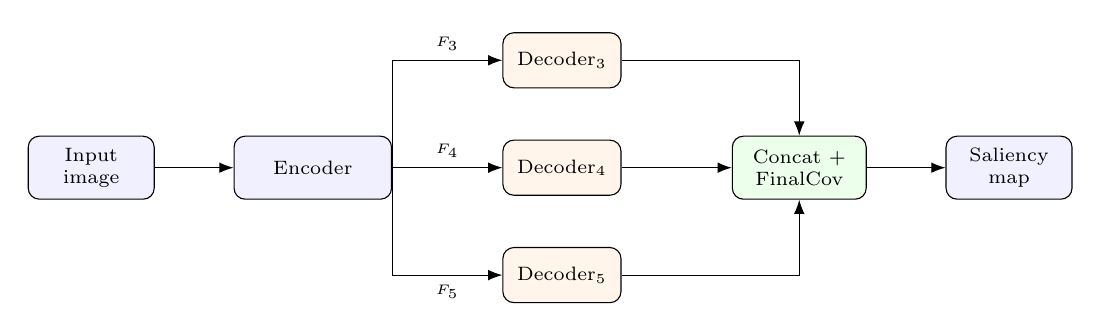
\begin{tikzpicture}[
  node distance=6mm and 10mm,
  block/.style={draw, rounded corners, minimum height=8mm, minimum width=16mm, align=center, font=\scriptsize, fill=blue!6},
  dec/.style={draw, rounded corners, minimum height=7mm, minimum width=15mm, align=center, font=\scriptsize, fill=orange!8},
  fuse/.style={draw, rounded corners, minimum height=8mm, minimum width=17mm, align=center, font=\scriptsize, fill=green!8},
  arr/.style={-{Latex[length=1.8mm]}, thin}
  ]
  \node[block] (in) {Input\\image};
  \node[block, right=of in, minimum width=20mm] (enc) {Encoder};
  \node[dec, above right=6mm and 14mm of enc] (d3) {Decoder$_3$};
  \node[dec, right=14mm of enc] (d4) {Decoder$_4$};
  \node[dec, below right=6mm and 14mm of enc] (d5) {Decoder$_5$};
  \node[fuse, right=14mm of d4] (fuse) {Concat +\\FinalCov};
  \node[block, right=of fuse] (out) {Saliency\\map};

  \draw[arr] (in) -- (enc);
  \draw[arr] (enc.east) |- node[pos=0.75, above, font=\tiny]{$F_3$} (d3.west);
  \draw[arr] (enc.east) -- node[above, font=\tiny]{$F_4$} (d4.west);
  \draw[arr] (enc.east) |- node[pos=0.75, below, font=\tiny]{$F_5$} (d5.west);
  \draw[arr] (d3.east) -| (fuse.north);
  \draw[arr] (d4.east) -- (fuse.west);
  \draw[arr] (d5.east) -| (fuse.south);
  \draw[arr] (fuse.east) -- (out.west);
\end{tikzpicture}
\caption{Pipeline shared by v1.1 and v2.0: an encoder taps three feature maps $F_3, F_4, F_5$ at increasing depth, each decoded independently and finally fused into a single saliency map. In v1.1 the encoder is a CNN trained from scratch (this section); in v2.0 it is a pretrained Swin-Tiny Transformer (\secref{sec:model20}).}
\label{fig:pipeline}
\end{figure}

\subsection{Encoder}
\label{subsec:encoder11}

The encoder is a VGG-style CNN trained from scratch: five blocks of $3{\times}3$ convolutions (stride 1, padding 1), batch normalization and ReLU; the first four blocks end with $2{\times}2$ max-pooling, the fifth does not, so the last two taps share spatial resolution. Feature maps are tapped after blocks 3, 4 and 5 (\tab{tab:encoder}) and passed to the three decoders below.

\begin{table}[t]
\centering
\caption{Encoder configuration (v1.1). $c$: output channels, $s$: stride relative to the input.}
\label{tab:encoder}
\begin{tabular}{@{}lllc@{}}
\toprule
\textbf{Block} & \textbf{Layers} & \textbf{Output} & \textbf{Tap} \\
\midrule
1 & Conv3-64, Conv3-64, MaxPool2 & $c{=}64,\,s{=}2$ & -- \\
2 & Conv3-128, Conv3-128, MaxPool2 & $c{=}128,\,s{=}4$ & -- \\
3 & (Conv3-256)$\times3$, MaxPool2 & $c{=}256,\,s{=}8$ & $F_3$ \\
4 & (Conv3-512)$\times3$, MaxPool2 & $c{=}512,\,s{=}16$ & $F_4$ \\
5 & (Conv3-512)$\times3$ & $c{=}512,\,s{=}16$ & $F_5$ \\
\bottomrule
\end{tabular}
\end{table}

\subsection{Decoders and fusion}
\label{subsec:decoder11}

Each feature map $F_k$ ($k\in\{3,4,5\}$) is processed by a dedicated decoder $D_k$ of identical structure: a $1{\times}1$ channel-reduction convolution, three blocks of $3{\times}3$ conv + BN + ReLU each interleaved with $\times2$ bilinear upsampling, and a final $1{\times}1$ conv + BN + ReLU collapsing to a single-channel map $S_k = D_k(F_k)$. The three maps are concatenated channel-wise and passed through \texttt{FinalCov}, a $1{\times}1$ (transposed) convolution followed by a sigmoid, giving the fused map
\begin{equation}
\label{eq:fuse}
S = \sigma\big(\mathrm{Conv}_{1\times1}\big([S_3;\,S_4;\,S_5]\big)\big) \in [0,1]^{H\times W}.
\end{equation}
Combining three independently-trained estimates, rather than relying on the deepest feature map alone, is what motivates the deep-supervision loss below: each branch must produce a plausible estimate on its own.

\subsection{Deep-supervision loss}
\label{subsec:loss11}

Let $P$ be a predicted map and $G$ the ground-truth fixation density, both normalized to sum to one. We combine three complementary terms: the Kullback-Leibler divergence
\begin{equation}
\label{eq:kld}
\mathrm{KLD}(G,P) = \sum_i G_i \log\left(\epsilon + \frac{G_i}{\epsilon + P_i}\right)\!,
\end{equation}
the linear correlation coefficient
\begin{equation}
\label{eq:cc}
\mathrm{CC}(G,P) = \frac{\mathrm{cov}(G,P)}{\sigma_G\,\sigma_P},
\end{equation}
and the histogram similarity
\begin{equation}
\label{eq:sim}
\mathrm{SIM}(G,P) = \sum_i \min(G_i, P_i),
\end{equation}
with $\epsilon$ a small constant avoiding division/log-of-zero in \eq{eq:kld}. These give a single per-map loss
\begin{equation}
\label{eq:single}
\mathcal{L}(G,P) = w_{\mathrm{kld}}\,\mathrm{KLD}(G,P) + w_{\mathrm{cc}}\big(1-\mathrm{CC}(G,P)\big) + w_{\mathrm{sim}}\big(1-\mathrm{SIM}(G,P)\big),
\end{equation}
with $w_{\mathrm{kld}} = w_{\mathrm{cc}} = w_{\mathrm{sim}} = 1$ throughout. Rather than applying \eq{eq:single} only to $S$, we apply \textit{deep supervision}, summing it over the fused map and all three branches:
\begin{equation}
\label{eq:total}
\mathcal{L}_{\mathrm{total}} = \mathcal{L}(G,S) + \sum_{k \in \{3,4,5\}} \mathcal{L}(G,S_k).
\end{equation}
This change was introduced in v1.0 (\secref{subsec:beta-v10}) to replace an initial MSE loss; together with Adam and batch normalization, it was the single change most responsible for the qualitative jump from Beta to v1.0.

\subsection{Dataset and training setup}
\label{subsec:training11}

The model is trained on SALICON~\cite{jiang2015salicon} (10{,}000 train / 5{,}000 validation images), resized to $240\times320$, tensor-converted without normalization or augmentation; MIT1003~\cite{judd2009learning} is held out entirely for test time (\secref{sec:validation}). \tab{tab:train11} lists the training configuration.

\begin{table}[t]
\centering
\caption{Training configuration, model v1.1.}
\label{tab:train11}
\begin{tabular}{@{}ll@{}}
\toprule
\textbf{Parameter} & \textbf{Value} \\
\midrule
Optimizer & Adam \\
Learning rate & $1\times10^{-3}$ \\
Batch size & 16 \\
Max.\ epochs & 150 \\
Early stopping & patience 15, $\Delta_{\mathrm{min}}=10^{-4}$ \\
Input resolution & $240\times320$ \\
Mixed precision & no \\
\bottomrule
\end{tabular}
\end{table}

% !TEX root = ../main.tex

\section{Model v2.0: Swapping in a Pretrained Transformer Encoder}
\label{sec:model20}

Model v2.0 follows the same pipeline as v1.1 (\fig{fig:pipeline}), using the decoders (\secref{subsec:decoder11}), fusion (\eq{eq:fuse}) and loss (\secref{subsec:loss11}) \textit{unchanged}. This section describes only what differs (the encoder and, consequently, the training configuration), consistent with isolating the effect of the encoder swap (\secref{subsec:v20-workflow}).

\subsection{Encoder}
\label{subsec:encoder20}

The scratch-trained VGG-style encoder of \secref{subsec:encoder11} is replaced with \texttt{swin\_tiny\_patch4\_window7\_224}, a Swin Transformer~\cite{liu2021swin} pretrained on ImageNet-1k, which merges shifted local-attention windows across four stages into a feature pyramid analogous to the v1.1 encoder's. We tap stages 2--4, giving $F_3, F_4, F_5$ with 192/384/768 channels at strides 8/16/32 (\tab{tab:encoder20}); inputs are resized to $224\times224$, the backbone's pretraining resolution.

\begin{table}[t]
\centering
\caption{Encoder configuration (v2.0, Swin-Tiny). $c$: output channels, $s$: stride relative to the input.}
\label{tab:encoder20}
\begin{tabular}{@{}llc@{}}
\toprule
\textbf{Stage} & \textbf{Output} & \textbf{Tap} \\
\midrule
2 & $c{=}192,\,s{=}8$  & $F_3$ \\
3 & $c{=}384,\,s{=}16$ & $F_4$ \\
4 & $c{=}768,\,s{=}32$ & $F_5$ \\
\bottomrule
\end{tabular}
\end{table}

Because $F_5$ now has stride 32 rather than 16 (\tab{tab:encoder}), Decoder$_5$ needs one extra $\times2$ upsampling stage to match v1.1's output resolution; Decoder$_3$/Decoder$_4$ are unaffected. All other decoder, fusion and loss components are identical to \secref{sec:model11}.

\subsection{Transfer learning and training setup}
\label{subsec:transfer20}
\label{subsec:training20}

To keep the pretrained representation intact while allowing some task-specific adaptation, the backbone is frozen by default and only its last stage is fine-tuned; the head is trained at a learning rate ten times higher than the unfrozen backbone stage, following standard differential-LR practice for fine-tuning on a much smaller target dataset. This is the most direct consequence of hypothesis (ii) in \secref{subsec:litreview}, left untested until this iteration. Since most of the backbone is frozen, memory pressure on the T4 GPU is dominated by head activations; we exploit this with a substantially larger batch size than v1.1, combined with automatic mixed precision (AMP). \tab{tab:train20} summarizes the configuration; dataset, splits and evaluation protocol are identical to v1.1 (\secref{subsec:training11}).

\begin{table}[t]
\centering
\caption{Training configuration, model v2.0. Parameters not listed are identical to \tab{tab:train11}.}
\label{tab:train20}
\begin{tabular}{@{}ll@{}}
\toprule
\textbf{Parameter} & \textbf{Value} \\
\midrule
Optimizer & Adam (2 param.\ groups) \\
Head learning rate & $3\times10^{-4}$ \\
Backbone learning rate & $3\times10^{-5}$ \\
Backbone freezing & frozen, last stage unfrozen \\
Batch size & 128 \\
Input resolution & $224\times224$ \\
Mixed precision & yes (AMP) \\
\bottomrule
\end{tabular}
\end{table}

% !TEX root = ../main.tex

\section{Test and Validation Protocol}
\label{sec:validation}

\subsection{Cross-dataset generalization test}
\label{subsec:crossdataset}

Both models are trained and early-stopped exclusively on SALICON splits (\secref{subsec:training11}); SALICON-only validation would measure in-distribution fit rather than genuine generalization. For a fair comparison we additionally evaluate both, for the first time, on MIT1003~\cite{judd2009learning}: 1{,}003 images with fixations from 15 observers, covering a substantially different distribution (general scenes, rather than SALICON's context-driven web imagery) never seen during training or model selection. The same preprocessing ($240\times320$ resize, no augmentation) and evaluation code are applied to both models on the same 1{,}003 images, so the comparison in \secref{sec:testing} isolates the encoder rather than pipeline differences.

\subsection{Evaluation metrics}
\label{subsec:metrics}

Saliency evaluation is sensitive to metric choice, since different metrics emphasize different map properties and a model can score well on one and poorly on another~\cite{bylinskii2019different}. We therefore report the same three complementary, distribution-based metrics used as loss terms in \secref{subsec:loss11}: KLD (\eq{eq:kld}, $\downarrow$), CC (\eq{eq:cc}, $\uparrow$) and SIM (\eq{eq:sim}, $\uparrow$), computed between the fused output $S$ and the MIT1003 ground truth, plus the total loss $\mathcal{L}_{\mathrm{total}}$ (\eq{eq:total}) used for checkpoint selection. Location-based metrics (AUC, NSS) are complementary but not yet part of our pipeline (\secref{sec:conclusions}).

\subsection{Model selection}
\label{subsec:selection}

For both models we test the checkpoint with the lowest SALICON validation loss observed before training stopped (\tab{tab:train11}). Neither run reached its early-stopping patience budget before being manually interrupted for practical (Colab session-length) reasons, so the numbers in \secref{sec:testing} reflect an as-yet incomplete training schedule and should be read as preliminary.

% !TEX root = ../main.tex

\section{Testing}
\label{sec:testing}

\noindent\textit{The numbers below are preliminary, from the best checkpoint of a manually-interrupted, not-yet-converged run (\secref{subsec:selection}); they stand in for the complete result set (full training curves and qualitative comparisons) to be added once final runs are completed.}

\subsection{Quantitative comparison}
\label{subsec:quant}

\tab{tab:results} reports the metrics of \secref{subsec:metrics} on MIT1003 for the best checkpoint of each model.

\begin{table}[t]
\centering
\caption{MIT1003 cross-dataset test results (best checkpoint, preliminary). $\downarrow$: lower is better, $\uparrow$: higher is better.}
\label{tab:results}
\begin{tabular}{@{}lcccc@{}}
\toprule
\textbf{Model} & $\mathcal{L}_{\mathrm{total}}\downarrow$ & KLD$\downarrow$ & CC$\uparrow$ & SIM$\uparrow$ \\
\midrule
v1.1 (CNN encoder)         & 7.6305 & 0.9229 & \textbf{0.6044} & \textbf{0.4809} \\
v2.0 (Swin-Tiny encoder)   & \textbf{7.5088} & 0.9436 & 0.5929 & 0.4609 \\
\bottomrule
\end{tabular}
\end{table}

\begin{figure}[t]
\centering
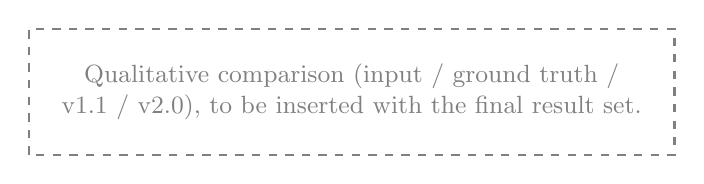
\begin{tikzpicture}
\draw[dashed, thick, gray] (0,0) rectangle (8.2,1.6);
\node[align=center, text width=7.4cm, font=\small, color=gray] at (4.1,0.8)
  {Qualitative comparison (input / ground truth / v1.1 / v2.0), to be inserted with the final result set.};
\end{tikzpicture}
\caption{Placeholder for the qualitative comparison figure.}
\label{fig:qual-placeholder}
\end{figure}

\subsection{Discussion}
\label{subsec:testdiscuss}

The two models are, at this stage, remarkably close: v2.0 reaches a marginally lower total loss, but v1.1 leads on all three individual metrics. Given how close the numbers are, we do not read this as a reliable ranking; it is consistent with our impression during development (\secref{subsec:v20-workflow}) that the pretrained Transformer encoder has not yet translated into a clear generalization advantage under the current training regime. We discuss possible explanations in \secref{sec:conclusions}.

% !TEX root = ../main.tex

\section{Concluding Remarks}
\label{sec:conclusions}

\subsection{Summary}
We presented the iterative development of a deep-supervised, multi-decoder saliency network: from a literal, from-scratch replica trained with MSE (Beta), through a modernized optimizer/normalization and a KLD/CC/SIM deep-supervision loss (v1.0), a higher-resolution refinement with early stopping (v1.1), to a hybrid model with a pretrained Swin-Tiny Transformer encoder in place of the CNN one, decoder/fusion/loss held fixed (v2.0). Both v1.1 and v2.0 were evaluated cross-dataset on MIT1003.

\subsection{Interpretation}
The largest single improvement across the project came from the v1.0 loss and optimization change, not from added capacity: both later iterations, higher resolution (v1.1) and a pretrained Transformer encoder (v2.0), delivered only marginal gains, despite v2.0 being, on paper, the most significant upgrade. Two, non-exclusive, explanations for the Transformer's limited impact: (i) the conservative differential learning rate and near-total backbone freezing (\secref{subsec:transfer20}) may not allow enough task-specific adaptation; (ii) both runs were manually interrupted before their early-stopping budget (\secref{subsec:selection}), so the comparison may not yet reflect fully-trained performance. Either way, this is a useful negative finding: swapping in a higher-capacity pretrained encoder is not, by itself, sufficient, since loss design, supervision strategy and training schedule jointly determine performance here.

\subsection{What we learned}
The loss function mattered more than any single architectural change, which reframed how we prioritized later iterations. A small, informal qualitative review (\secref{subsec:beta-v10}) was a cheap, effective sanity check, and cross-dataset testing (\secref{sec:validation}) was necessary to avoid over-trusting in-distribution numbers. Working under a hard hardware constraint (one T4 GPU) forced choices such as backbone freezing, mixed precision and batch size, which materially affected the very comparison we set out to make.

\subsection{Limitations and future work}
The results in \secref{sec:testing} are preliminary and both models should be retrained to convergence before drawing firm conclusions on v1.1 vs.\ v2.0. Natural next steps: unfreezing more Transformer stages or sweeping the differential learning rate; adding data augmentation and input normalization (currently absent, \secref{subsec:training11}); extending evaluation with location-based metrics (AUC, NSS) alongside KLD/CC/SIM; and producing the qualitative figures and full training curves still placeholders in this draft.


\bibliography{biblio}
\bibliographystyle{ieeetr}

\end{document}
